\appendix

\section*{Appendix}

\section{Bridge from mismatch discovery to mediation}
\label{sec-app-bridge}

An early motivating question was whether a sparse feature pair could repair
a grammatical mismatch while preserving the planned noun token. On a source
prompt of the form ``Someone who treats eye diseases is,'' suppressing a
competing feature pair crossed the decision boundary from majority
\texttt{a} toward \texttt{an} while preserving \texttt{ophthalmologist}
on that prompt. The held-out transfer of the same frozen pair did
\emph{not} behave as a noun-preserving grammar tool: many expected-\texttt{a}
controls flipped toward \texttt{an}, and noun tokens changed on 37/107
prompts, with zero grammar-only repairs that kept the noun fixed
(Figure~\ref{fig-generalization} in the main text).

That failure sharpened the question from ``can we fix articles?'' to
``do Latent-Planning-style dual-effect interventions identify separable
noun-token control, or can free-generation noun changes be explained by
mediation through the generated article?'' Behavioral article-recall
baselines on this 270M stack strongly prefer majority \texttt{a}; reliable
\texttt{an} when required by listed targets is rare---consistent with
\citet{hanna2026latent}'s scale story. Subsequent main-text assays address
that sharpened question.

\section{Reproducibility map}
\label{app:reproducibility}

Experiment directories under \texttt{experiments/} contain
\texttt{config.json}, \texttt{run.py}, \texttt{results/summary.json}, and
\texttt{results/report.md}. Key assays:

\begin{center}
\small
\begin{tabular}{ll}
\toprule
Assay & Directory \\
\midrule
Fixed-pair held-out transfer & \texttt{fixed\_pair\_generalization/} \\
Free-generation dual-effect GoF & \texttt{planning\_gain\_content\_clincher/} \\
Selection-criterion ablation (S1--S4) & \texttt{selection\_criterion\_ablation/} \\
Dose--response & \texttt{planning\_dose\_response/} \\
Forced content-lock / dual & \texttt{forced\_content\_lock/} \\
Causal tetrad on twins & \texttt{trajectory\_causal\_tetrad/} \\
Selective \(b\)-step + force-native & \texttt{selective\_bc\_force\_native/} \\
Fixed \(b\), intervention-on-at-\(c\) & \texttt{causal\_edge\_independence/} \\
Per-noun LP-style under fixed \(b\) & \texttt{per\_noun\_fixed\_b\_c\_to\_c/} \\
Residual MLP-in under fixed \(b\) & \texttt{residual\_direction\_fixed\_b\_c\_to\_c/} \\
Near-boundary screen + oracle patch & \texttt{fixed\_b\_positive\_control/} \\
\bottomrule
\end{tabular}
\end{center}

Environment: conda Python with PyPI \texttt{circuit-tracer}; model and
transcoder snapshots as recorded in each \texttt{config.json}. Experiments
ran on one Apple M1 (16~GB RAM) workstation with CPU inference; attribution
runs dominate wall-clock time (typically tens of minutes per graph).

\section{Additional selection details}
\label{app:selection}

S1--S3 are selected from intersection of article and future-content
attribution graphs at position \(P\), with article direct-effect bounds for
S3. Per-noun assays select top-4 features per family by target direct
effect (and by target--source contrast) subject to
\(|\mathrm{DE}(a/an)|\le 0.05\). Residual assays unit-normalize
per-layer MLP-in differences before scaling by \(\alpha\). Oracle
positive-control patches blend source and target MLP-in activations at
layers \(\{8,10,12,14\}\) under fixed native \(b\).

\section{Per-noun fixed-\texorpdfstring{\(b\)}{b} null plot}
\label{app:pernoun}

\begin{figure}[t]
\centering
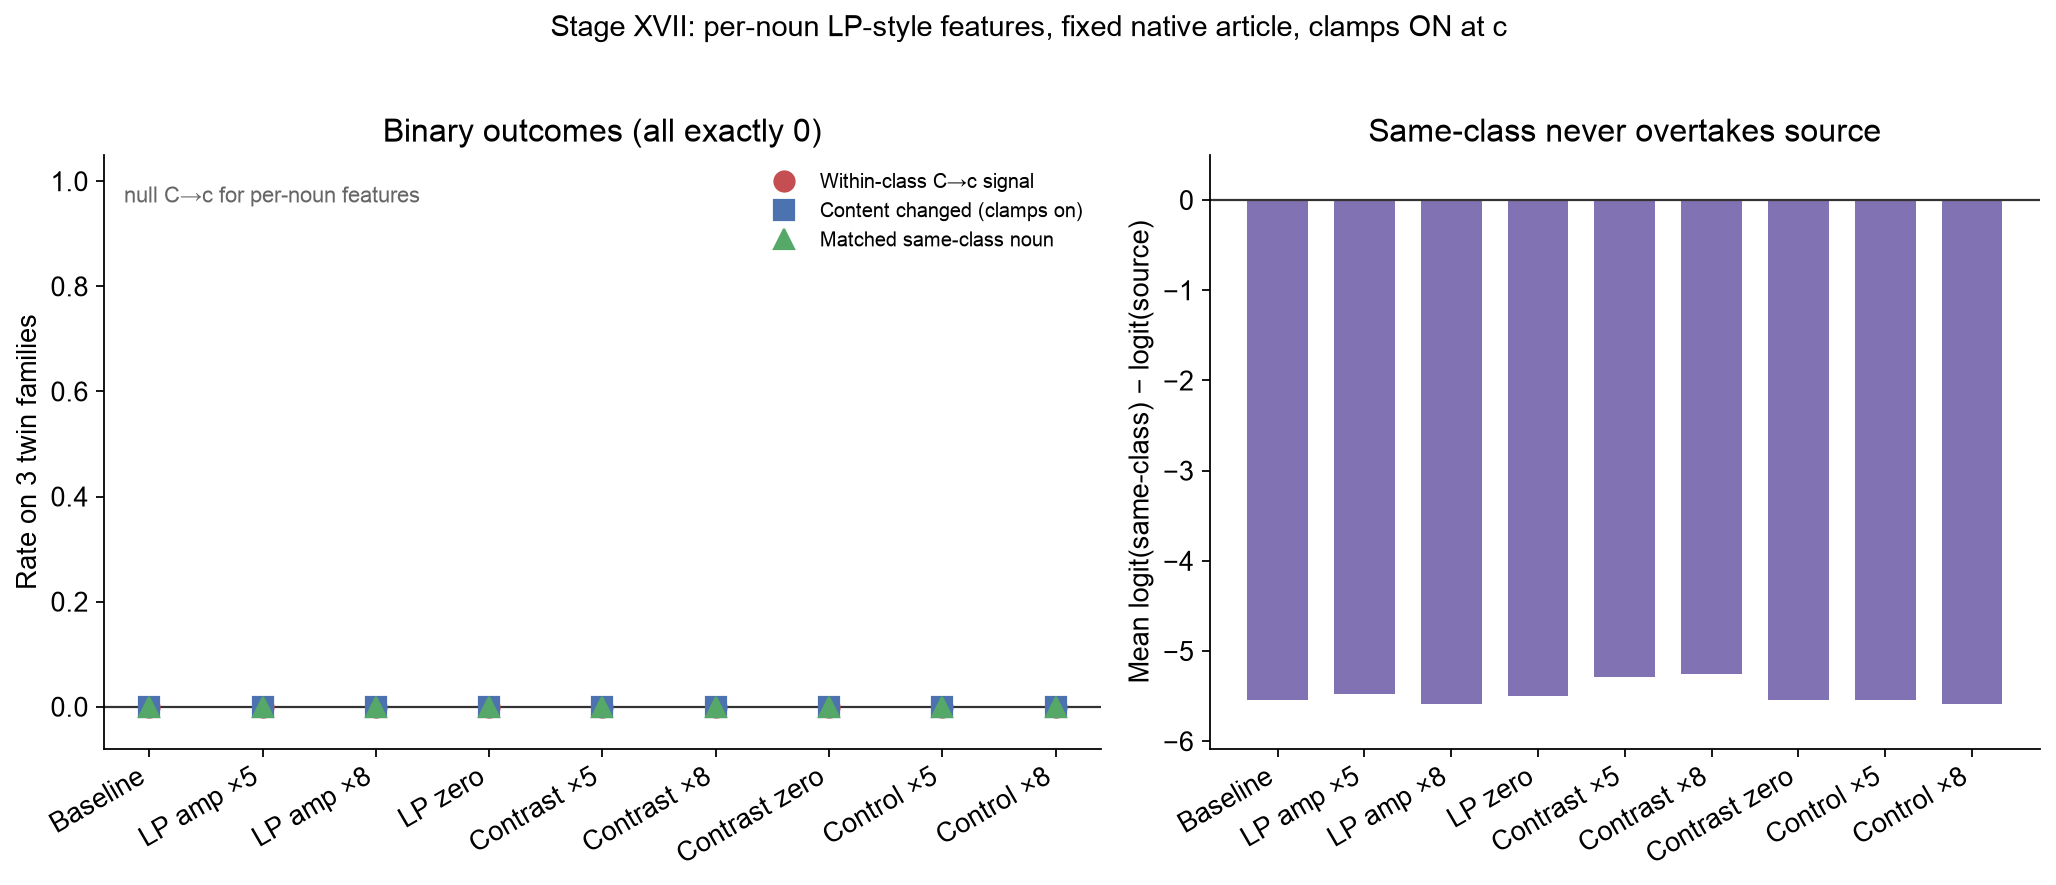
\includegraphics[width=0.92\linewidth]{docs/collaborator-report/figures/figure10_per_noun_fixed_b.png}
\caption{Per-noun LP-style and contrast features under fixed \(b\):
within-class top-1 outcomes remain zero; same-class nouns stay \(\sim 5\)
logits below source. Visually parallel to the main-text fixed-\(b\) panel
(Figure~\ref{fig-fixed-b}); rates are summarized in
Table~\ref{tbl-handles}.}
\label{fig-pernoun}
\end{figure}

For completeness we include the per-noun plot. Binary within-class top-1
outcomes are exactly zero across LP-target, contrast, and control
amplify/zero arms on the three twin families; the same-class logit gap
stays near \(-5\). The main text emphasizes continuous effects, floor
limits, and the failed MLP-in oracle positive control rather than stacking
near-identical all-zero panels.

\section{Oracle positive-control details}
\label{app:oracle}

\begin{table}[t]
\centering
\caption{Oracle MLP-in activation patching under fixed \(b\) versus random
controls. Continuous effects are tiny; top-1 target matches remain zero.}
\label{tbl-oracle}
\small
\begin{tabular}{lccc}
\toprule
Mix \(\lambda\) & Oracle match (\(N{=}4\)) & Oracle mean \(\Delta\Delta\) [95\%] & Random mean \(\Delta\Delta\) (\(N{=}20\)) \\
\midrule
0.25 & 0.00 & \(0.06\,[-0.01,0.13]\) & \(-0.03\,[-0.09,0.04]\) \\
0.50 & 0.00 & \(0.03\,[-0.03,0.09]\) & \(-0.11\,[-0.22,0.01]\) \\
0.75 & 0.00 & \(0.03\,[-0.03,0.09]\) & \(-0.06\,[-0.22,0.09]\) \\
1.00 & 0.00 & \(0.06\,[-0.01,0.13]\) & \(-0.04\,[-0.19,0.10]\) \\
\bottomrule
\end{tabular}
\end{table}

Near-boundary screening identified
\texttt{scientist}/\texttt{biologist} (\(-0.75\) logits) and
\texttt{scientist}/\texttt{chemist} (\(-1.13\)). Oracle patches blend
source and target MLP-in activations at layers \(\{8,10,12,14\}\) under
fixed native \(b\). The construction does not produce top-1 target matches
and does not clearly beat matched-norm random controls, so it fails as an
assay-validation positive control on this stack.
